\chapter{Progettazione e codifica}
\label{cap:progettazione-codifica}

\intro{Breve introduzione al capitolo}\\

\section{Tecnologie e strumenti}
\label{sec:tecnologie-strumenti}

Di seguito viene data una panoramica delle tecnologie e degli strumenti utilizzati per sviluppare il progetto.
\subsection{Python}
Python offre diverse librerie utili per l'apprendimento automatico, il trattamento del linguaggio naturale e molto altro ancora.
\subsection{Jupiter Notebook}
Applicazione che permette di creare documenti testuali contenenti anche codice eseguibile. Utile per realizzare e documentare analisi di dati.
\subsection{Tika}
\label{subsec:tika}
Tika è un tool che permette di estrarre dai file i suoi metadata (come titolo del file, autore e altro) e il suo contenuto sottoforma di testo (strutturato e non).
Riesce ad estrarre i dati da molti formati tra cui Pdf, docx e html.
\subsection{Pandas}
\label{subsec:pandas}
Pandas è una libreria che fornisce strutture dati e strumenti per la manipolazione e l'analisi dei dati.
Il primo passo importante dell'estrazione delle tabelle dai vari documenti è stato quello di avere un DataFrame a disposizione con i valori di quest'ultime. 
Pandas è stato utilizzato per l'estrazione delle tabelle dai file in formato html e docx.
\subsection{PdfPlumber}
\label{subsec:pdfplumber}
PdfPlumber è una libreria per Python che fornisce funzionalità per l'estrazione automatizzata di testo e tabelle dai documenti PDF.
Nel progetto è stato utilizzato per estrarre le tabelle dai vari pdf.
\subsection{Python-docx}
\label{subsec:python-docx}
Python-docx è una libreria che consente di creare, modificare e leggere documenti Microsoft Word.
Grazie a questa libreria è possibile manipolare le tabelle presenti all'interno dei file docx.
\subsection{BeautifulSoup}
\label{subsec:beautifulsoup}
BeautifulSoup è una libreria Python che facilita l'estrazione di dati da file HTML e XML.
Consente, inoltre, di creare e modificare tag all'interno del codice con il quale si sta lavorando.
\subsection{OpenAI API}
API fornita da OpenAI tramite la quale si possono sfruttare i vari modelli offerti per la generazione di testo in linguaggio naturale.
\subsection{Weaviate}
\label{subsec:weav}
Weaviate è un database vettoriale utile per la ricerca dei dati basata sulla loro semantica e sulle loro relazioni. 

\section{Progettazione e codifica}
\label{sec:progettazione-codifica}
La parte di codice sviluppata per questo progetto integra la parte di logica dell'applicazione di un backend già esistente.

\begin{figure}[!h]
    \centering
    \scalebox{0.5}{
        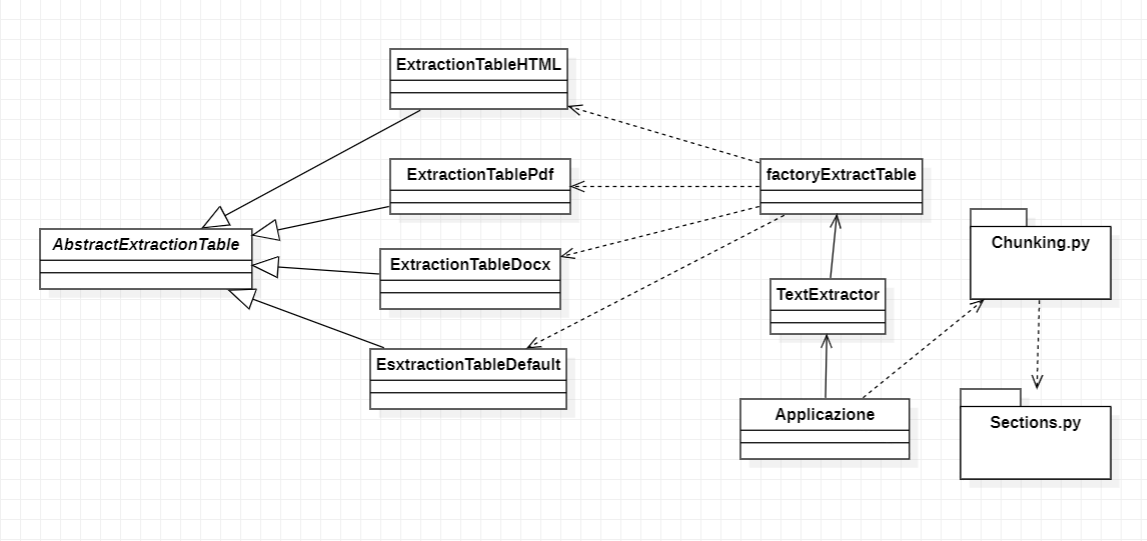
\includegraphics{images/architettura.png}
    }
    \caption{Architettura della parte di codice implementata nel backend}
\end{figure}

\subsection{L'idea}
Grazie a Tika riusciamo a convertire il contenuto dei documneti in XHTML in modo tale da poter lavorare con del testo strutturato.
Con i documenti dove c'è già una struttura al di sotto Tika riesce a convertire molto bene il contenuto dei documenti in un XHTML ed è in grado di individuare intestazioni (e i loro livelli gerarchici h1,h2,...), tabelle e altro.
Per questo non è stato difficile riuscire a implementare le funzioni utili per lavorare con i file HTML e Docx.
Per i Pdf invece le cose sono state più complesse, gli unici tool individuati che riescono a convertire bene il contenuto dei pdf (come "Aspose") in testo strutturato richiedono una licenza a pagamento e quindi è stato utilizzato comunque Tika.
In questo caso il contenuto viene rappresentato tramite dei tag \emph{div} che rappresentano le singole pagine e il contenuto stesso viene trascritto tramite dei tag \emph{p}. \\

\noindent Qui di seguito vengono descritte le parti di codice sviluppate di maggiore rilevanza.

\subsection{ExtractionTable}
ExtractionTableHTML, ExtractionTableDocx, ExtractionTablePdf e ExtractionTableDefault implementano la classe AbstractExtractionTable ed espongono quelle funzioni utili alle operazioni da fare sulle tabelle presenti nei documenti di quello specifico formato:
\begin{itemize}
    \item La funzione \textbf{extractTable} prende in ingresso un file path e restituisce la lista delle tabelle, convertite in DataFrame, presenti nel documento indicato nel percorso. Per estrarre le tabelle sono stati utilizzati i seguenti tool:
    \begin{itemize}
        \item HTML: \nameref{subsec:pandas};
        \item Docx: \nameref{subsec:python-docx};
        \item Pdf: \nameref{subsec:pdfplumber};
    \end{itemize}
    \item La funzione \textbf{replaceTable} prende in ingresso un file path, una lista di tabelle da sostituire all'interno del documento e ritorna la versione XHTML del documento estratta tramite \nameref{subsec:tika} con le tabelle linearizzate sostituite all'interno.
    Per HTML e Docx la funzione rimane uguale: grazie a \nameref{subsec:beautifulsoup} è possibile cercare tutti i vari tag \emph{table} e sostituire il loro contenuto. Per i Pdf invece sono state usate le espressioni regolari per cercare e sostituire le tabelle. 
    \item Le tabelle vengono linearizzate tramite la funzione \textbf{adaptTable} che prende in ingresso un DataFrame e ritorna la stringa che rappresenta la tabella.
\end{itemize} 

\subsection{FactoryExtractTable}
Viene presentata una funzione \textbf{factoryExtractTable} che prende in ingresso un file path e in base al suo formato istanzia un oggetto di tipo ExtractionTable.
Quando viene inserito un file in un formato che non corrisponde a uno dei tre principali viene instanziato un oggetto di tipo ExtractionTableDefault.
Si è deciso di sviluppare questa classe per avere comunque delle possibilità nella sostituizione delle tabelle nel caso in cui si riesce a convertire discretamente il documento in XHTML.

\subsection{TextExtractor}
TextExtractor mette a disposizione la funzione \textbf{extractText} che prende in ingresso un file path e un booleano \emph{getText}.
Questa funzione ritorna:
\begin{itemize}
    \item Con getText = False, il contenuto del documento convertito in XHTML;
    \item Con getText = True, il contenuto del documento convertito il stringa (testo non strutturato). 
\end{itemize}

Per lavorare più facilmente con il contenuto XHTML prodotto dalla conversione dei pdf, al \emph{body} viene aggiunto un primo titolo \emph{h1} con contenuto il nome del file come primo tag e vengono estratti tutti i tag da dentro i \emph{div} che rappresentano le pagine (individuabili con BeautifulSoup perchè hanno \emph{"class=page"}).

\subsection{Sections.py}
Modulo creato che contiene funzioni utili per convertire un XHTML in una struttura ad albero rinominata "Sezione"

La Sezione viene definita in base ai vari titoli dei paragrafi e al loro livelo gerarchico ed è formata dai seguenti campi:
\begin{itemize}
    \item titolo (stringa): titolo della sezione;
    \item contenuto (lista): all'interno della lista ci può essere sia contenuto testuale che altre sezioni. 
\end{itemize}

La funzione che viene esposta per creare la Sezione si chiama \textbf{makeSection} e prende in ingresso contenuto in forma XHTML.

\subsection{Chunking.py}
Modulo creato che contiene funzioni utili per la conversione delle Sezione in Chunk.

Il Chunk è formato dai seguenti campi:
\begin{itemize}
    \item titolo (stringa): titolo della chunk;
    \item parentsTit (lista di stringhe): contiene tutti i titoli superiori in senso gerarchico al paragrafo;
    \item contenuto (stringa): porzione di contenuto del paragrafo.
    \item page (intero): numero della pagina da dove è stato preso il contenuto del chunk (ancora non utilizzato, messo per successivi aggiornamenti del codice). 
\end{itemize}

Le funzioni esposte e utili all'esterno di questo modulo sono le seguenti:
\begin{itemize}
    \item La funzione \textbf{chunking} che prende in ingresso il contenuto XHTML di un documento, il numero massimo di token da cui può essere composto un chunk, la funzione di encode da testo in token e la funzione di decode da token a testo.
    Questa funzione sfrutta makeSection (definita in Section.py) e restituisce la lista ordinata di chunk che compongono il documento.
    All'interno della funzione viene chiamata anche la funzione \textbf{cleanText} effettua la pulizia del testo rimuovendo le ripetizioni dei caratteri passati come input.
    \item La funzione \textbf{createTitleForChunk} crea la stringa di titoli unita in base a un numero massimo di token da cui può essere composta, prende una lista di titoli e il numero di token che possono comporre la stringa.
    Questa funzione non ha senso di essere applicata sui documenti nei quali Tika non riesce a riconoscere una struttura: viene trovato un unico titolo che è il nome del file e sostanzialmente è come se fosse tutto sotto un unico paragrafo.
\end{itemize}

\subsection{Applicazione}
La parte dell'applicazione effettiva in questo momento è implementata tramite un Jupiter Notebook ed è il prototipo che mi è stato passato all'inizio dello stage.
Quello che ho fatto è stato chiamare le varie funzioni per ottenere le tabelle linearizzate e il chunking migliorato all'interno.
La procedura che viene eseguita per far funzionare il prototipo è la seguente:
\begin{enumerate}
    \item Viene dato un insieme di documenti;
    \item Ogni documento convertito in XHTML tramite \textbf{extractText} che a sua volta linearizza le tabelle;
    \item Vengono creati i chunk tramite la funzione \textbf{chunking};
    \item I vari chunk vengono caricati sul motore di ricerca;
    \item Quando viene posta una domanda, vengono restituiti i 10 chunk con lo score più alto (hybrid search);
    \item La richiesta (domanda + 10 chunk) viene consegnata al Chat-Completion Model che elabora le informazioni e restituisce una risposta alla domanda. 
\end{enumerate}

\section{Design pattern}

Per strutturare il codice in maniera tale da renderlo di facile manutenzione ed estensione sono stati usati i \gls{design pattern}\glsfirstoccur.
Il design pattern utilizzato è stato lo \textbf{\gls{strategy}}\glsfirstoccur: per ogni formato dei file l'estrazione della tabella avviene in maniera differente quindi viene applicato lo strategy pattern che definisce una classe astratta \emph{AbstractExtractionTable} che verrà poi implementata a seconda del formato preso in cosiderazione. 
